\documentclass[10pt]{article}
\usepackage{icmlko}

\icmlmeta{IP 파운데이션 월드모델}{348}{묶음을 풀었다}{서랍의 마지막 둘 --- 하나는 버리고 하나는 갈랐더니 판이 처음으로 12/12 로 올랐다}

\begin{document}

\twocolumn[
\icmlheader

\begin{abstract}
노트 347이 \texttt{fund\_cat} 을 서랍에서 꺼내 펀딩 $+$0.0964 를 얻고
``서랍을 마저''를 남겼다. 남은 둘에 검사 ⑤ 를 돌렸다.

\begin{center}\footnotesize
\begin{tabular}{lrrl}
\hline
서랍 & 검사 ⑤ 판 & 양수 & \\
\hline
\texttt{anime\_medium}(321) & $-$0.0026 & \textbf{0/8} & \textbf{버린다} \\
원천 축 \textbf{열}(324) & $-$0.0003 & 4/8 & 묶음으로는 안 된다 \\
\hline
\end{tabular}
\end{center}

\textbf{\texttt{anime\_medium} 은 미리 적은 대로 떨어졌다} --- 검사 ④를
아슬하게 통과했지만 최빈 밖이 6\%뿐이라 잡음과 구별이 안 된다(노트 335).

\textbf{원천 축 열은 묶음으로는 0 인데 도메인별로는 갈린다} --- 펀딩
$+$0.0893(8/8) · 모바일 $+$0.0109(7/8) 대 세계애니 $-$0.0011(3/8).
\textbf{그래서 이긴 도메인의 축만 남겼다}(\texttt{fund\_maxprice} ·
\texttt{mob\_advisory} · \texttt{mob\_ngenre} · \texttt{mob\_nlang}).

\begin{center}\small
\begin{tabular}{lrr}
\hline
 & 검사 ⑤ 판 & 실제 \\
\hline
열 다 & $-$0.0003 (4/8) & --- \\
\textbf{이긴 넷} & \textbf{$+$0.0082 (8/8)} & \textbf{$+$0.0068 (12/12)} \\
\hline
\end{tabular}
\end{center}

\textbf{판 0.4763 $\to$ 0.4815 이고 열 도메인이 하나도 안 내려간다}
--- 펀딩 $+$0.0521(12/12) · 모바일 $+$0.0135(12/12) · 도서
$+$0.0135(11/12) · 시장팝업 $+$0.0264 · 팝업 $+$0.0091 · 아이돌 $+$0.0065 ·
게임 $+$0.0027. \textbf{이 실험실에서 판이 12/12 로 오른 첫 처치다.}

\textbf{지는 여섯이 이기는 넷을 덮고 있었다.} 노트 324가 열을 묶음으로 재고
판 $-$0.0027 을 보고 서랍에 넣었는데, \textbf{그 안에 $+$0.0068 이 들어
있었다.}
\end{abstract}
]

\section{서랍의 마지막 둘}

\begin{figure*}[t]
\centering
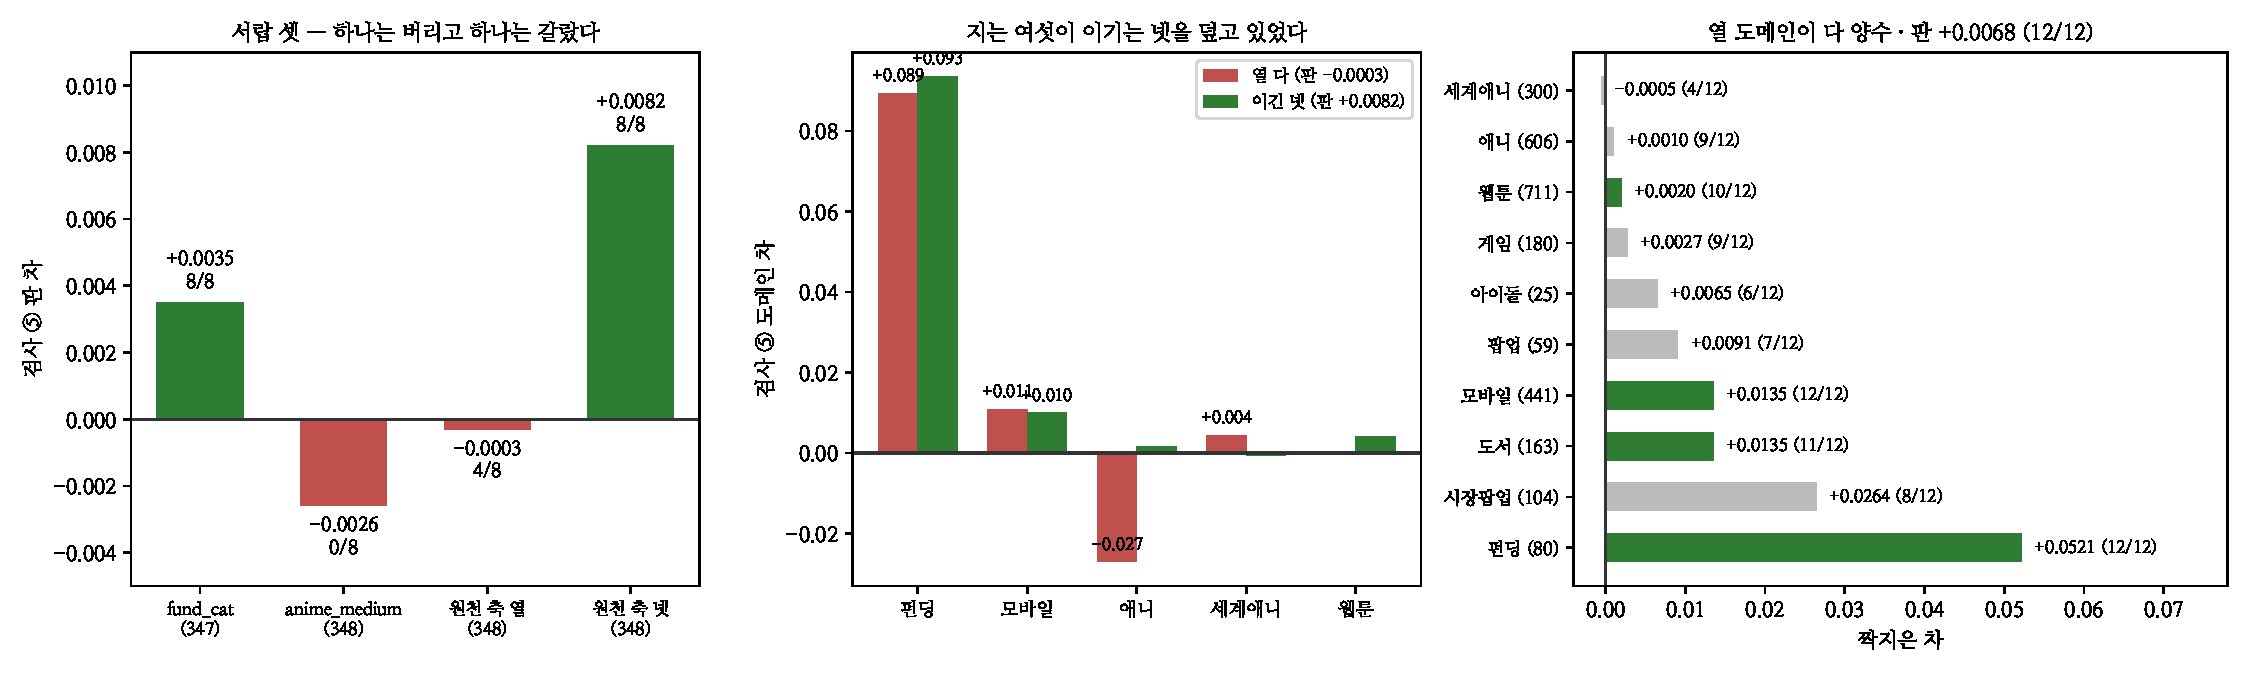
\includegraphics[width=\textwidth]{figs/bundle.pdf}
\caption{왼쪽 --- 서랍 넷의 검사 ⑤. 가운데 --- 묶음과 넷의 도메인별.
오른쪽 --- 붙인 결과.}
\end{figure*}

\begin{center}\footnotesize
\begin{tabular}{llr}
\hline
축 & 그때(노트) & 오늘 검사 ⑤ \\
\hline
\texttt{fund\_cat} & $+$0.0023 (309) & $+$0.0035 (8/8) \\
\texttt{anime\_medium} & $+$0.0000 (321) & $-$0.0026 (0/8) \\
원천 축 열 & $-$0.0027 (324) & $-$0.0003 (4/8) \\
\textbf{원천 축 넷} & --- & \textbf{$+$0.0082 (8/8)} \\
\hline
\end{tabular}
\end{center}

\section{묶음이 감춘 것}

\begin{center}\footnotesize
\begin{tabular}{lrr}
\hline
도메인 & 열 다 & 이긴 넷 \\
\hline
\textbf{펀딩} & $+$0.0893 & $+$0.0935 \\
\textbf{모바일} & $+$0.0109 & $+$0.0100 \\
세계애니 & $-$0.0011 & --- \\
\hline
판 & $-$0.0003 & \textbf{$+$0.0082} \\
\hline
\end{tabular}
\end{center}

\textbf{펀딩 · 모바일의 값은 거의 안 변한다}(0.089$\to$0.094 · 0.011$\to$
0.010). 바뀐 것은 \emph{판}이다 --- 나머지 여섯 축(애니 둘 · 세계애니 셋 ·
웹툰 하나)이 각자 조금씩 물던 열값이 사라졌다. \textbf{노트 339가 잰
``잡음 축이 끼치는 해''가 여기서 $-$0.0085 로 보인다.}

\section{붙였다}

\begin{center}\footnotesize
\begin{tabular}{lrrr}
\hline
 & 평균 & SD & 양수 \\
\hline
\textbf{펀딩} & \textbf{$+$0.0521} & 0.0266 & \textbf{12/12} \\
시장팝업 & $+$0.0264 & 0.0679 & 8/12 \\
\textbf{모바일} & \textbf{$+$0.0135} & 0.0071 & \textbf{12/12} \\
도서 & $+$0.0135 & 0.0136 & 11/12 \\
팝업 & $+$0.0091 & 0.0164 & 7/12 \\
아이돌 & $+$0.0065 & 0.0306 & 6/12 \\
게임 & $+$0.0027 & 0.0054 & 9/12 \\
\hline
\textbf{판} & \textbf{$+$0.0068} & 0.0028 & \textbf{12/12} \\
\hline
\end{tabular}
\end{center}

\textbf{내려간 도메인이 없다.} 배포 규칙 ②는 ``어느 도메인도 문턱 밖으로
안 내려간다''인데 \textbf{아무도 안 내려갔다.} 이 창에서 잰 처치 중
처음이다.

\paragraph{검사 ⑤ 네 번째} 예측 $+$0.0082 · 실제 $+$0.0068. 네 사례가
$+$0.0042/$+$0.0041 · $+$0.0027/$+$0.0015 · $+$0.0035/$+$0.0030 ·
$+$0.0082/$+$0.0068 이다 --- \textbf{네 번 다 방향이 맞고 크기가
0.6$\sim$1.0배다.}

\section{남은 것}
\begin{center}\footnotesize
\begin{tabular}{ll}
\hline
갈래 & 왜 \\
\hline
\textbf{묶음을 다 풀어 보라} & 태그 · 위키 · 검색도 도메인별로 \\
지는 여섯을 하나씩 & 애니 둘이 왜 해로운가 \\
검사 ⑤ 를 규약에 & 네 번 맞혔다 \\
서랍이 또 있나 & 세 번 열어 둘을 건졌다 \\
\hline
\end{tabular}
\end{center}

\paragraph{규약} \textbf{묶음으로 재고 묶음으로 버리지 마라.} 노트 324가
원천 축 열을 한 번에 붙여 판 $-$0.0027 을 보고 ``검사는 거르지 줄 세우지
못한다''로 끝냈다. \textbf{그 판정은 묶음에 대해서만 맞았다} --- 안에
펀딩 $+$0.09 와 모바일 $+$0.01 이 들어 있었고 여섯이 그것을 덮고 있었다.
\textbf{그리고 그것을 볼 수 있게 한 것은 검사 ⑤ 의 도메인별 답이다} ---
판 하나로는 묶음 안을 못 본다.

\end{document}
